\chapter{Criação de redes simples -- \textit{Cross-over}, \textit{hub} e \textit{switch}}\label{chp:redesSimples}

Neste capítulo, vamos ver como criar uma rede bem simples, de um computador para outro (um \textit{notebook}) de uma forma direta na \Cref{sec:conexDireta}. Depois, vamos criar uma pequena rede local (\textit{Local Area Network} -- LAN) um pouco mais complexa, com mais computadores conectados. 

Para as redes mais complexas vamos usar, primeiro, um \textit{hub}, para implementar a topologia barramento na \Cref{sec:conexHub}. Depois, usando um \textit{switch}, vamos implementar a topologia estrela na \Cref{sec:conexSwitch}. 
Não esqueça de executar o \CPT para realizar os exercícios a seguir.

\section{Conexão direta entre computadores}\label{sec:conexDireta}

Para estabelecer uma conexão direta entre dois computadores, precisamos criar um ambiente com dois desses dispositivos (um PC e um \textit{laptop}) e um cabo \textit{cross-over}. Para tanto, execute os passos a seguir.

\begin{enumerate}[label*=\arabic*.]
    \item Adicione um PC e um \textit{laptop} (\textit{End Devices}) no seu ambiente, arrastando os respectivos ícones para a área em branco.
    \item Dentre as conexões (\textit{Connections}), selecione um cabo \textit{cross-over}; depois, ligue o PC ao \textit{laptop}. 
    \begin{enumerate}[label*=\arabic*.]
       \item Ao estabelecer a conexão, escolha a interface física \enquote{\textit{Fast ethernet}} em ambos os dispositivos.
    \end{enumerate}
\end{enumerate}

A \Cref{fig:conexaoCrossover} mostra como deve ficar a tela no \CPT após a realização desse primeiro passo. Note que os triângulos verdes próximos a cada dispositivo indicam que eles estão conectados.

\begin{figure}
    \centering
    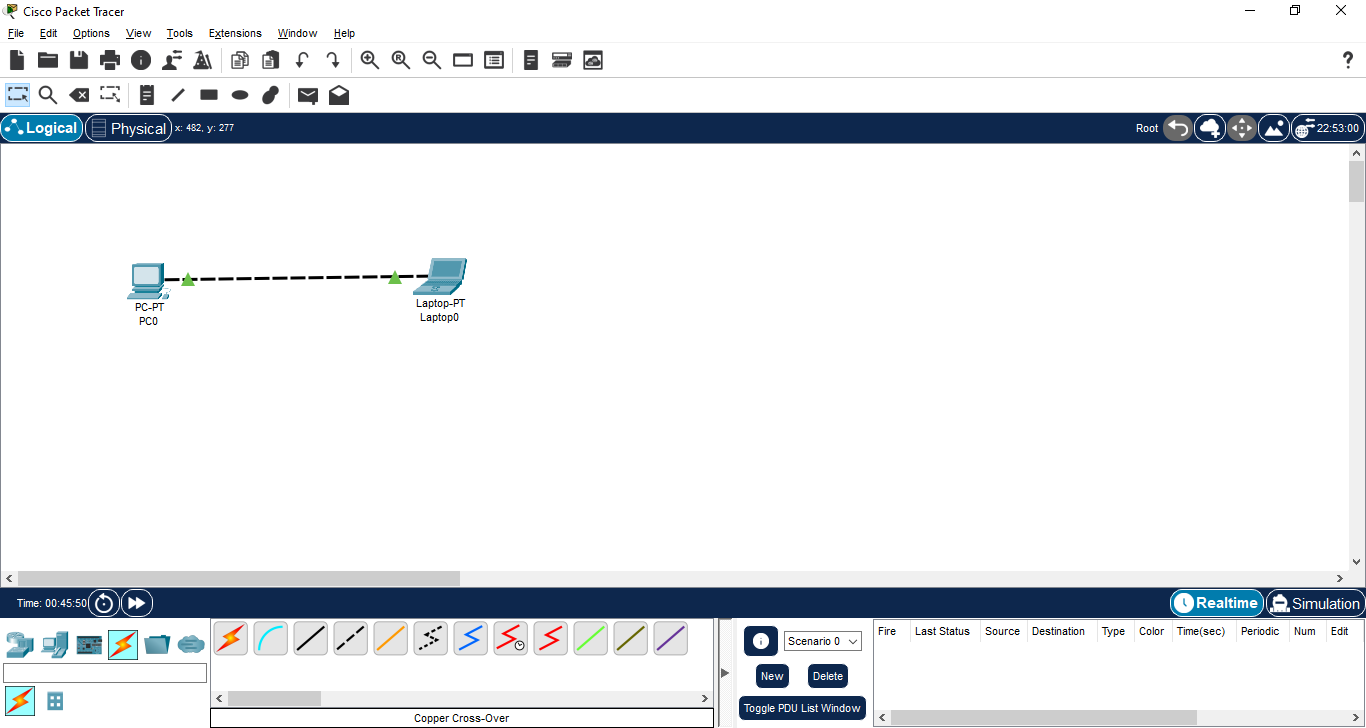
\includegraphics[width=.99\textwidth]{Figuras/ConexaoCrossover}
    \caption{Conexão direta com cabo \textit{cross-over}.}\label{fig:conexaoCrossover}
\end{figure}

Vamos agora realizar uma configuração estática básica para a conexão desses computadores. Para isso, siga os seguintes passos:

\begin{enumerate}
    \item Clique no dispositivo.
    \item Na parte superior da nova janela aberta, clique na opção \textit{Desktop}.
    \item Selecione o ícone em que está escrito \textit{IP Configuration}.
    \item Na caixa de texto em que está escrito \textit{IPv4 Address}, informe o endereço IP do dispositivo (veja quais são a seguir).
\end{enumerate}

Nesse caso, utilizaremos o IP \texttt{10.0.0.5} para o PC e o IP \texttt{10.0.0.6} para o \textit{laptop}. Perceba que, após a inserção do endereço IP, a máscara \texttt{255.0.0.0} é automaticamente inserida também.

\subsection{Verificação da conexão entre os componentes}\label{subsec:verificaConex}
Vejamos agora se ambos os componentes conseguem trocar dados. Para isso utilizaremos o comando \Comando{ping}. execute os passos a seguir:

\begin{enumerate}
    \item Clique em um dos dispositivos (por exemplo, o PC).
    \item Na parte superior da nova janela aberta, clique na opção \textit{Desktop}.
    \item Selecione o ícone em que está escrito \textit{Command Prompt}.
    \item Execute o comando a seguir e veja o resultado.
    \begin{lstlisting}[style=MyBashStyle]
ping 10.0.0.6
    \end{lstlisting}
\end{enumerate}

\section{Exercício}
Repita o mesmo procedimento anterior, dessa vez para o \textit{laptop}. Não esqueça que, nesse caso, você deve informar para o comando \Comando{ping} o endereço IP do PC (\texttt{10.0.0.5}).

Apenas como ilustração, tente informar um endereço IP de um dispositivo que não existe ainda nessa rede (por exemplo, \texttt{10.0.0.7}).

\section{Conexão de vários computadores com um \textit{hub}}\label{sec:conexHub}
Vamos criar uma pequena rede local com três computadores (PCs), interligados por um \textit{hub}. Essa rede formará uma topologia do tipo barramento. Para tanto, execute os passos a seguir.

\begin{enumerate}[label*=\arabic*.]
    \item Adicione três PCs no seu ambiente, arrastando os respectivos ícones para a área em branco.
    \item Adicione  um \textit{hub} (\textit{Network Device}) no seu ambiente.
    \item Dentre as conexões, selecione um cabo de cobre (par trançado); depois, ligue cada um dos PCs ao \textit{hub}. 
    \begin{enumerate}[label*=\arabic*.]
       \item Ao estabelecer a conexão, escolha a interface física \enquote{\textit{Fast ethernet}} em ambos os dispositivos.
    \end{enumerate}
    \item Configure os endereços IP de cada um dos PCs (\texttt{10.0.0.5}, \texttt{10.0.0.6} e \texttt{10.0.0.7}) e a máscara \texttt{255.0.0.0}.
\end{enumerate}

Feita a configuração, verifique usando o comando \Comando{ping}, se todos os computadores estão acessíveis, um a partir do outro. Para isso, use o procedimento da \Cref{subsec:verificaConex}. A \Cref{fig:hub} ilustra a topologia criada.

\begin{figure}
    \centering
    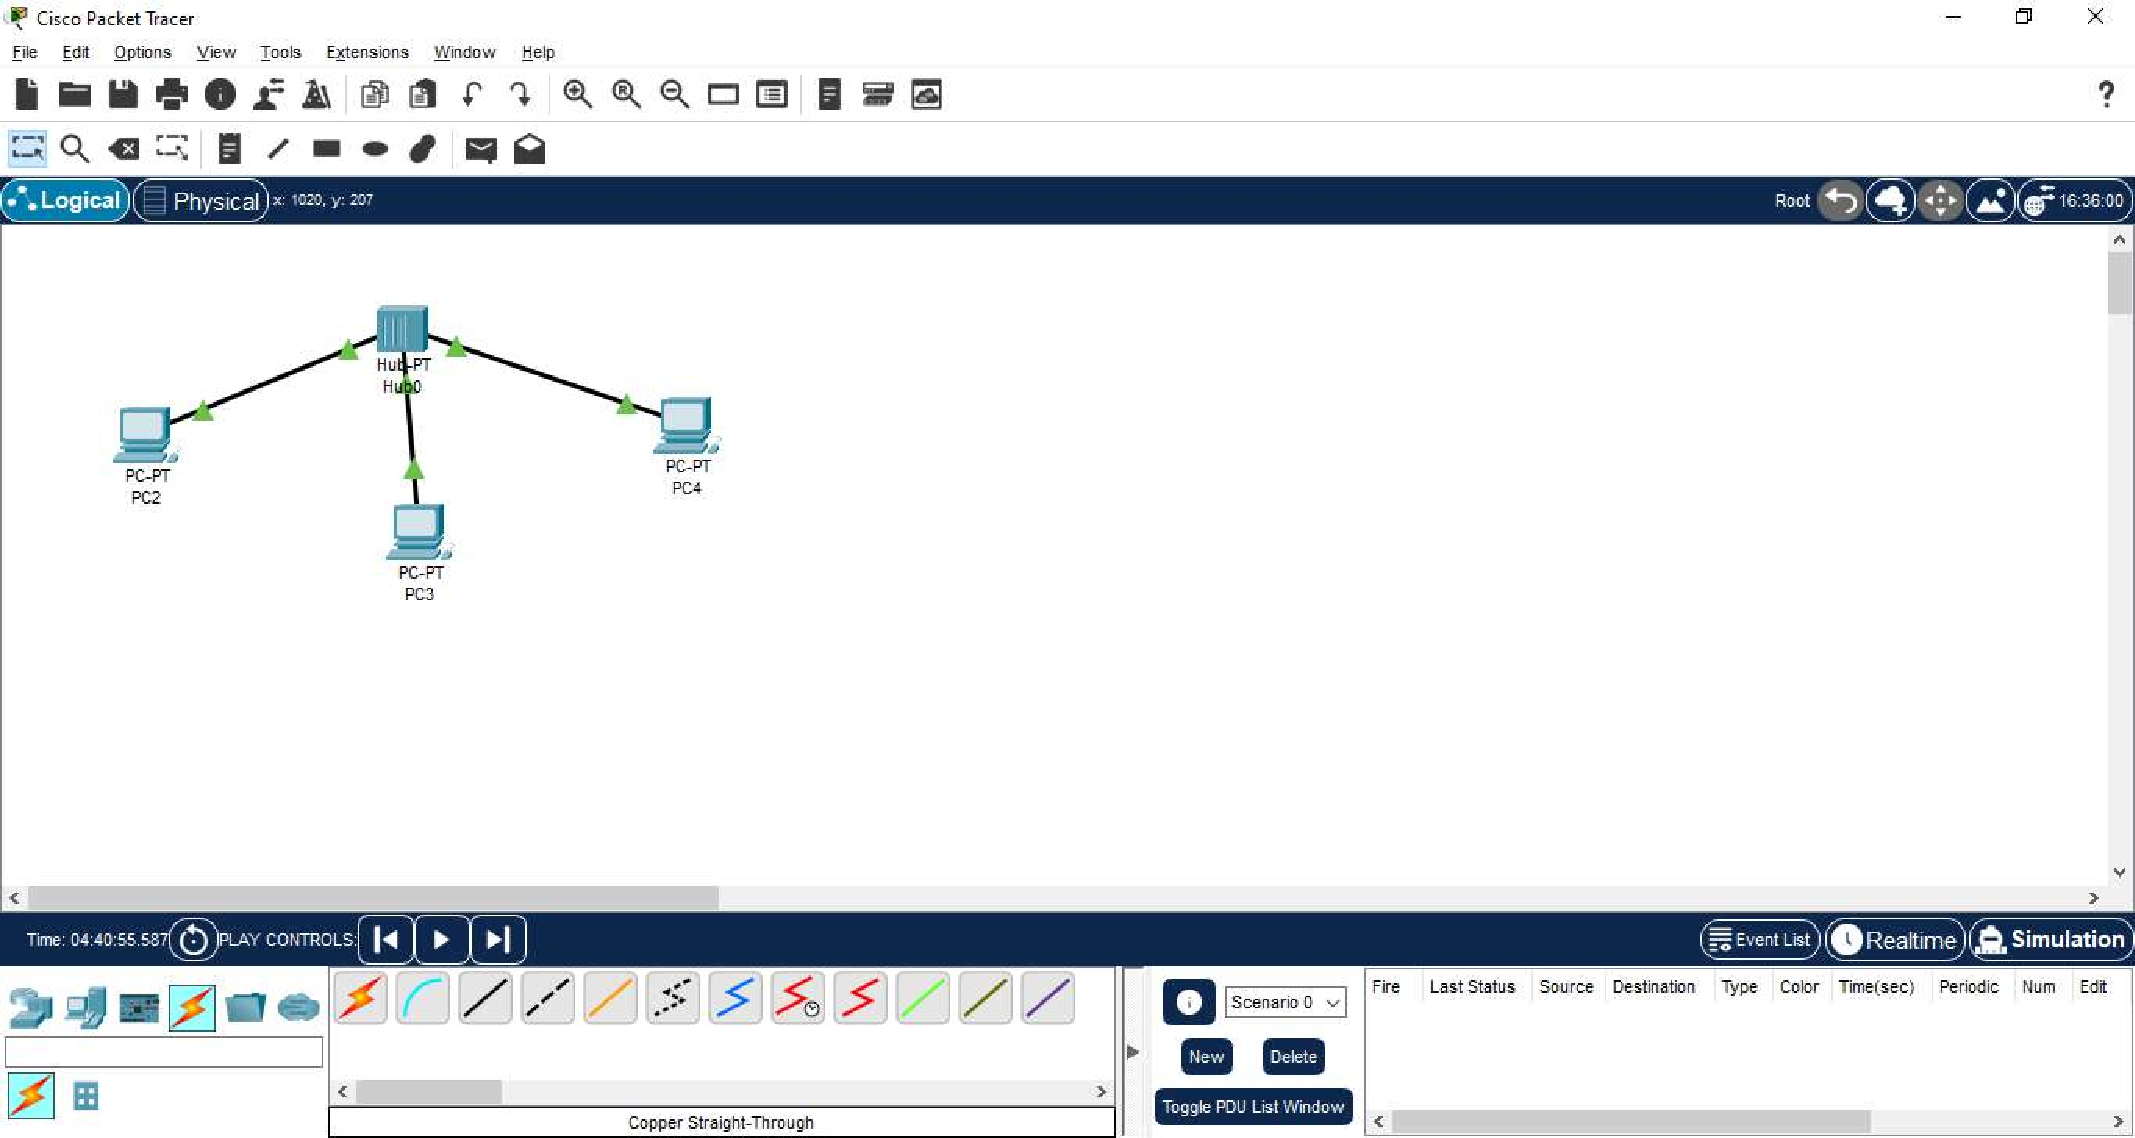
\includegraphics[width=.99\textwidth]{Figuras/hub}
    \caption{Topologia de barramento com hub.}
    \label{fig:hub}
\end{figure}

\subsection{Troca de dados entre os computadores}\label{subsec:trocaPDUs}
Veremos agora a troca de dados entre os nós (computadores) de uma rede. Chamaremos esses dados de \textit{Protocol Data Unit} (PDU). Na verdade, a PDU é a unidade básica de troca entre entidades que se comunicam usando um protocolo de rede específico.

Para simular o envio de PDUs usando a topologia de barramento, vamos executar os seguintes passos.

\begin{enumerate}[label*=\arabic*.]\label{enum:envioPDU}
    \item Selecione uma PDU simples, representada pelo ícone \faIcon[regular]{envelope} na barra de ferramentas. Você verá que o ponteiro do \textit{mouse} mudou para o mesmo ícone. Agora, você vai determinar a origem e o destino do PDU.
    \begin{enumerate}[label*=\arabic*.]
        \item Leve o ponteiro do \textit{mouse} a um dos PCs (por exemplo, o \texttt{PC0}) e clique sobre ele. Essa será a origem.
        \item Depois, leve o ponteiro do \textit{mouse} a outro dos PCs (por exemplo, o \texttt{PC2}) e clique sobre ele. Esse será o destino.
    \end{enumerate}
    
    \item Terminados os passos anteriores, vamos à simulação. Clique no botão de simulação (\textit{Simulation}) no canto inferior direito.

    \item Na nova janela que se abrir, clique no ícone \textit{play} (\faPlay) para rodar a simulação e observe o que acontece.
    \begin{enumerate}[label*=\arabic*.]
        \item Note que o PDU saiu da origem e foi encaminhado para todos os nós da rede. Porém, apenas o nó de destino confirmou seu reconhecimento (\textit{acknowledge}).
        \item O PDU de reconhecimento também foi enviado a todos os nós, mas apenas o nó destino o recebeu corretamente. Os demais nós descartaram a PDU que não era para eles.
     \end{enumerate}
\end{enumerate}

\section{Conexão de vários computadores com um \textit{switch}}\label{sec:conexSwitch}
Agora, vamos substituir o \textit{hub} por um \textit{switch}, para criar uma rede local com topologia estrela. Execute os passos a seguir.

\begin{enumerate}[label*=\arabic*.]
        \item Remova o \textit{hub}, clicando no ícone \faIcon{backspace} na barra de ferramentas e, em seguida, clicando sobre o \textit{hub}.
        \item No canto inferior esquerdo, dentre os dispositivos de rede (\textit{Network Devices}), selecione os \textit{switches}. Dentre os \textit{switches}, selecione o 2960.
        \item Agora, para cada um dos computadores, usando os cabos par trançados, execute os seguintes passos:
          \begin{enumerate}[label*=\arabic*.]
            \item Ligue a interface \textit{Fast Ethernet} do computador à interface \texttt{Fast Ethernet0/?} do \textit{switch}. Note que o 0 significa a VLAN 0. No lugar da `?', substitua por um número diferente (indicando que é outra interface do \textit{switch}).

            \item Aguarde um tempo até que o \textit{switch} resolva todas as conexões.

            \item Verifique se os computadores ainda estão com os mesmos endereços IP configurados (\texttt{10.0.0.5}, \texttt{10.0.0.6} e \texttt{10.0.0.7}) e máscara \texttt{255.0.0.0}.

            \item Verifique se todos os computadores estão visíveis entre si com o comando \Comando{ping}.
          \end{enumerate}
\end{enumerate}

Depois de terminada a configuração, repita a simulação descrita na \Cref{subsec:trocaPDUs}.

\section{Exercício}
Terminada as simulações nas \Cref{sec:conexHub,sec:conexSwitch}, quais foram as diferenças entre ambas as simulações?  O que acontece com as PDUs original e \textit{acknowledge} nas redes?  Por que dizemos que uma rede local interligada com um \textit{switch} tem uma topologia estrela?